\section{Core Language}	
Zombie works on a untyped, purely functional, call by value language. Program in the language is then executed by the CEK abstract machine.

The CEK machine is an transition system between states. In other words, given a state, the CEK machine formalize what that state might transit into. Running a program under the CEK machine then correspond to transiting the machine until it reach a non-transitable state.

A state in the CEK machine is consisted of 3 parts:

\begin{enumerate}
	\item \textcolor{blue}{C}ontrol, the expression currently being evaluated.
	\item \textcolor{blue}{E}nvironment, a name-key map of free variable of Control.
	\item \textcolor{blue}{K}ontinuation, which will be invoked when Control is evaluated.
\end{enumerate}

Our formalization of the CEK machine alternate between two mode.

It start with the step mode, which break down a complex expression, focusing on a part of it, storing the other parts onto the continuation, until it find an atomic expression, then convert the atomic expression into a value, and call the other mode, apply.

The apply mode transform the values according to the continuation, giving back control to step once there is more expression to evaluate.

The machine start with a special continuation, Done, and end when Value V is being applied to the Done continuation. This denote that the original expression evaluate to value V.

We had deliberately chosen to represent our semantic by the CEK machine, as it have three crucial properties:

\begin{enumerate}
	\item It is deterministic. Given any state, it can transit to at most 1 state.
	
	\item It is linear. An execution of a program can be characterized as a (possibly infinite) sequence the abstract machine transit through.
	
	\item Each step take a small, bounded amount of work, and especially for lookup/alloc.
\end{enumerate}
\begin{figure}
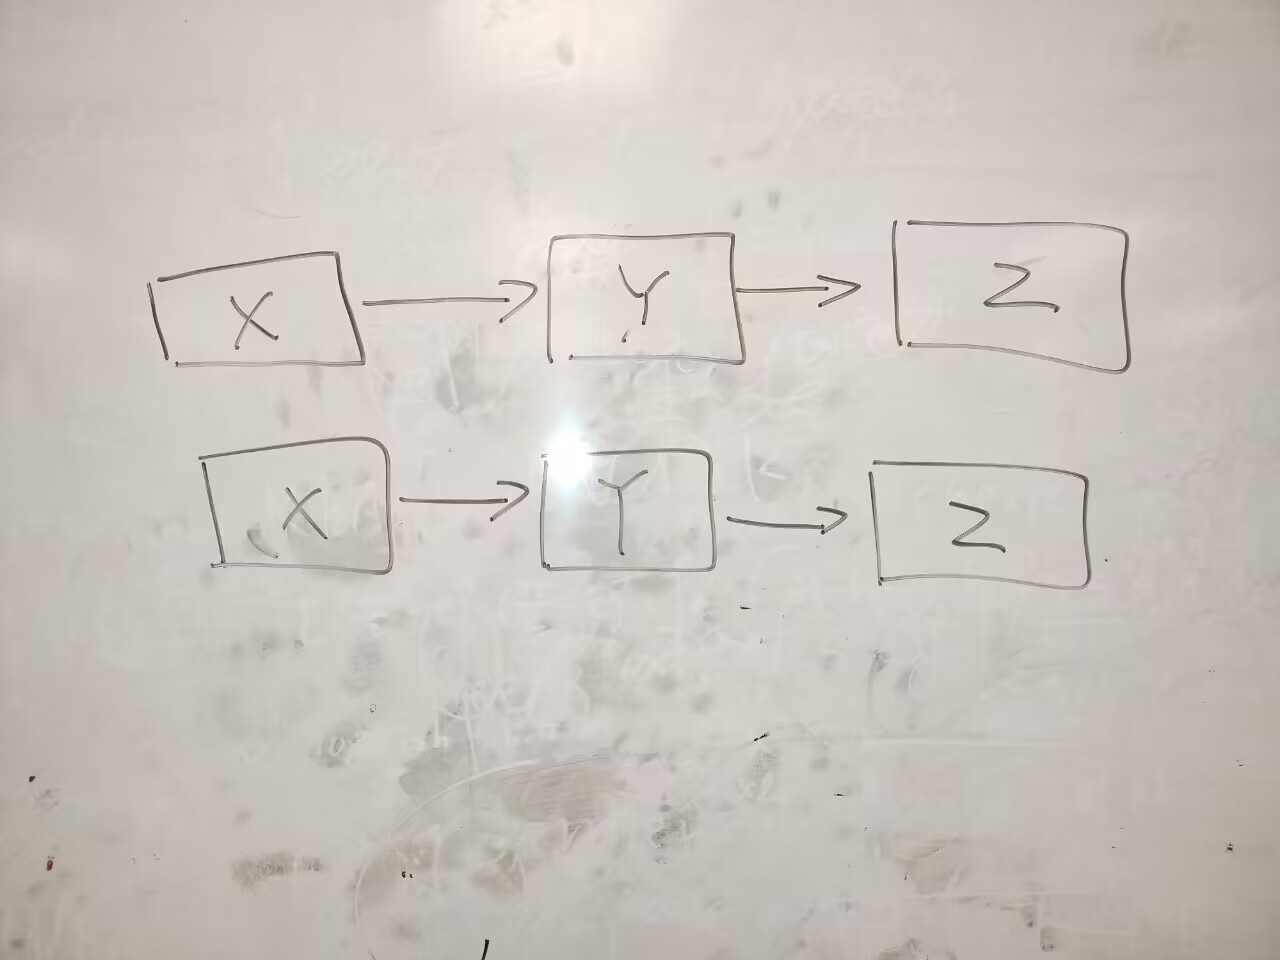
\includegraphics[width=0.5\columnwidth]{0}
\caption{the deterministic, linear nature of the CEK machine}
\end{figure}
\begin{figure}
	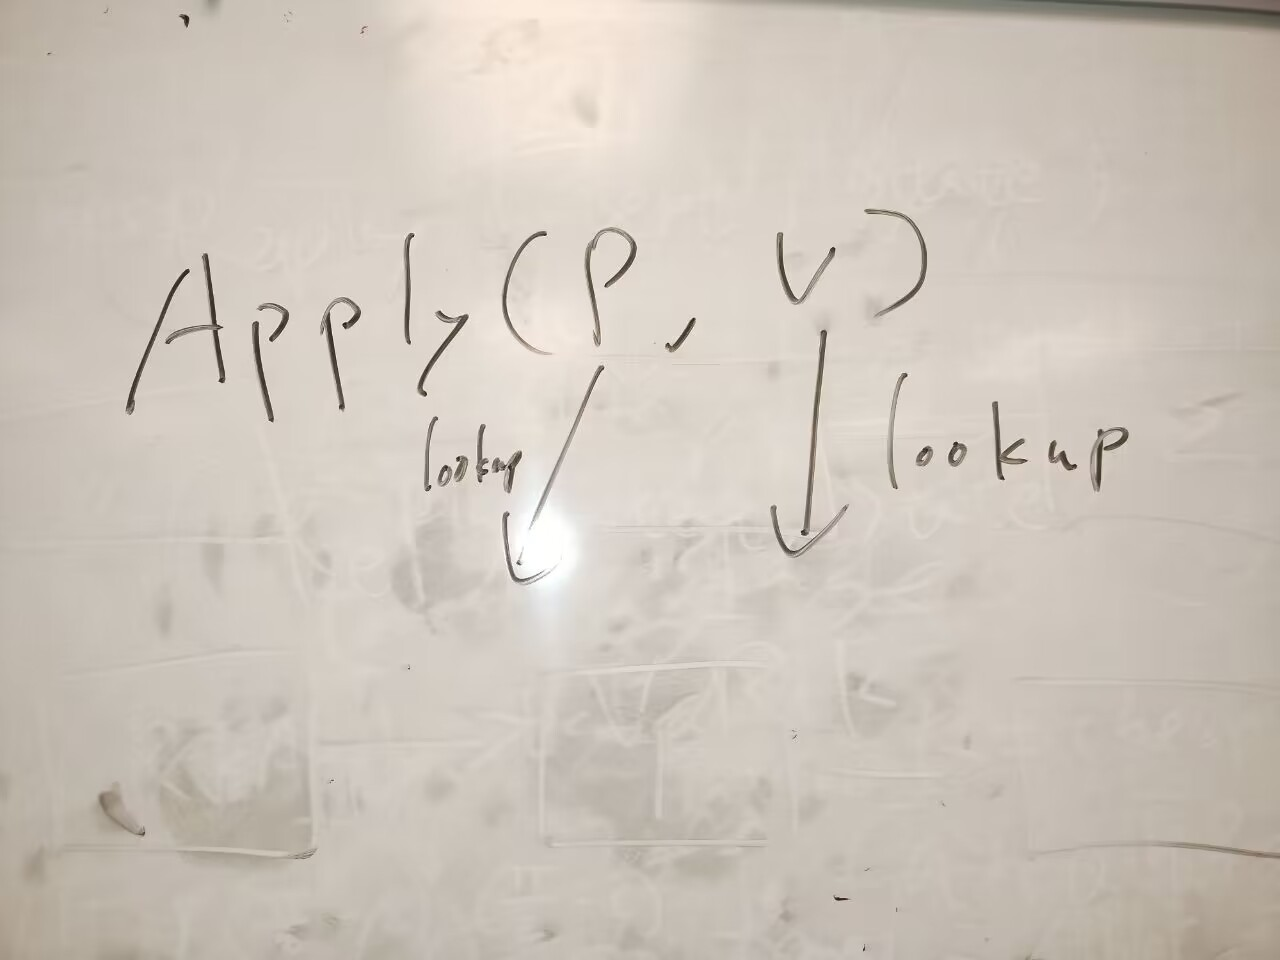
\includegraphics[width=0.5\columnwidth]{1}
	\caption{the machine does a small constant amount of pointer lookup}
\end{figure}
Note how our implementation is different from a CEK Machine: In particular, we had made pointers and pointer lookup explicit, as we later have to abstract over and reason over them. 
Similarly, allocation is now explicit as well.

Below we sketch out the language and the cek machine. Note that this is the standard semantic - there is neither uncomputation nor replaying present. Uncomputation will be represented independently afterward.

\newcommand{\mytableshape}{p{6em} p{2.6em} p{1em} p{0.45\textwidth}}
\begin{figure}
	\begin{tabular}{\mytableshape}
		Name & $N$ & $::=$ & A set of distinct names \\
		Expr & $E$ & $::=$ & $
		N \mid
		\sLet~N~E~E \mid
		\sLam~N~E \mid
		\sApp~E~E \mid
		\sProd~E~E \mid
		\sZro~E \mid
		\sFst~E \mid
		\sLeft~E \mid
		\sRight~E \mid
		\sCase~E~N~E~N~E $
	\end{tabular}
	\caption{The source language}
\end{figure}

\begin{figure}
	\begin{tabular}{\mytableshape}
		Heap & $H$ & $::=$ & An abstract key value store \\
		Pointer$\langle X \rangle$ & $P\langle X \rangle$ & $::=$ & Key into heap with value type $X$ \\
		Alloc & & : & $(X, H) \to (\text{Pointer}\langle X \rangle, H)$ \\
		Lookup & & : & $(\text{Pointer}\langle X \rangle, H) \to X$ \\
	\end{tabular}
	\caption{Heap API}
\end{figure}

\begin{figure}
	\begin{tabular}{\mytableshape}
		Continuation & $K$ & $::=$ & $P \langle \KCell \rangle$ \\
		
		KCell & & $::=$ & $
		\Done \mid
		\KLet~N~\Env~E~K \mid
		\KApp_0~\Env~E~K \mid
		\KApp_1~V~K \mid
		\KProd_0~\Env~E~K \mid
		\KProd_1~V~K \mid
		\KZro~K \mid
		\KFst~K \mid
		\KLeft~K \mid
		\KRight~K \mid
		\KCase~\Env~N~E~N~E~K $ \\
		
		Value & $V$ & $::=$ & $P\langle \VCell \rangle$ \\
		VCell & & $::=$ & $
		\Clos~\Env~N~E \mid
		\VProd~V~V \mid
		\VLeft~V \mid
		\VRight~V $ \\
		
		Environment & $\Env$ & ::= & $(N, V) \dots$ \\
		State & & ::= & $\Step~E~\Env~K \mid \Apply~K~V $ \\
	\end{tabular}
	\caption{Definitions for the CEK Machine}
\end{figure}

\begin{figure}
	\begin{mathpar}
		\inferrule{ }{\text{State}, H \leadsto \text{State}, H} \and
		\inferrule{ }{\Step(N, \Env, K), H \leadsto \Apply(K, \Env(N)), H} \and
		\inferrule{\Alloc(\KLeft~K, H) = (P, H')}{\Step(\sLeft~X, \Env, K), H \leadsto \Step(X, \Env, P), H'} \and
		\inferrule{\Alloc(\KRight~K, H) = (P, H')}{\Step(\sRight~X, \Env, K), H \leadsto \Step(X, \Env, P), H'} \and
		\inferrule{\Alloc(\KProd_0~K~R, H) = (P, H')}{\Step(\sProd~L~R, \Env, K), H \leadsto \Step(L, \Env, P), H'} \and
		\inferrule{\Alloc(\KZro~K, H) = (P, H')}{\Step(\sZro~X, \Env, K), H \leadsto \Step(X, \Env, P), H'} \and
		\inferrule{\Alloc(\KFst~K, H) = (P, H')}{\Step(\sFst~X, \Env, K), H \leadsto \Step(X, \Env, P), H'} \and
		\inferrule{\Alloc(\KCase~\mathit{LN}~L~\mathit{RN}~R~\Env, H) = (P, H')}{\Step(\sCase~X~\mathit{LN}~L~\mathit{RN}~R, \Env, K), H \leadsto \Step(X, \Env, P), H'} \and
		\inferrule{\Alloc(\KLet~A~K~C~\Env, H) = (P, H')}{\Step(\sLet~A~B~C, \Env, K), H \leadsto \Step(B, \Env, P), H'} \and
		\inferrule{\Alloc(\KApp_0~K~X, H) = (P, H')}{\Step(\sApp~F~X, \Env, K), H \leadsto \Step(F, P), H'} \and
		\inferrule{\Alloc(\Clos~\Env(\text{fv})\cdots N~E, H) = (P, H')}{\Step(\sLam~N~E, \Env, K), H \leadsto \Apply(K, P), H'}
	\end{mathpar}
	\caption{Abstract Machine Transition: Step}
\end{figure}

\begin{figure}
	\begin{mathpar}
		\inferrule{\Lookup(P, H) = \KLeft~K \and \Alloc(\VLeft~V, H) = (P', H')}{\Apply(P, V), H \leadsto \Apply(K, P'), H'} \and
		\inferrule{\Lookup(P, H) = \KRight~K \and \Alloc(\VRight~V, H) = (P', H')}{\Apply(P, V), H \leadsto \Apply(K, P'), H'} \and
		\inferrule{\Lookup(P, H) = \KCase~\Env~\mathit{LN}~L~\mathit{RN}~R~K \and \Lookup(V, H) = \VLeft~V}{\Apply(P, V) \leadsto \Step(L, \Env(\mathit{LN} := V), K)} \and
		\inferrule{\Lookup(P, H) = \KCase~\Env~\mathit{LN}~L~\mathit{RN}~R~K \and \Lookup(V, H) = \VRight~V}{\Apply(P, V) \leadsto \Step(R, \Env(\mathit{RN} := V), K)} \and
		\inferrule{\Lookup(P, H) = \text{KProd0}~\Env~R~K \and \Alloc(\KProd_1~V~\Env~K, H) = (P', H')}{\Apply(P, V), H \leadsto \Apply(K, P'), H'} \and
		\inferrule{\Lookup(P, H) = \KProd_1~L~K \and \Alloc(\VProd~L~V, H) = (P, H')}{\Apply(P', V), H \leadsto \Apply(K, P'), H'} \and
		\inferrule{\Lookup(P, H) = \KZro~K \and \Lookup(V, H) = (\VProd~X~Y)}{\Apply(P, V), H \leadsto \Apply(K, X), H'} \and
		\inferrule{\Lookup(P, H) = \KFst~K \and \Lookup(V, H) = (\VProd~X~Y)}{\Apply(P, V), H \leadsto \Apply(K, Y), H'} \and
		\inferrule{\Lookup(P, H) = \KLet~A~\Env~C~K}{\Apply(P, V), H \leadsto \Step(C, \Env(A := V), K), H'} \and
		\inferrule{\Lookup(P, H) = \KApp_0~\Env~X~K \and \Alloc(\KApp_1~V~K, H) = (P', H')}{\Apply(P, V), H \leadsto \Step(X, \Env, P'), H'} \and
		\inferrule{\Lookup(P, H) = \KApp_1~F~K \and \Lookup(F, H) = (\Clos~\Env~N~E, H)}{\Apply(P, V), H \leadsto \Step(E, \Env(N := V), K), H'}
	\end{mathpar}
	\caption{Abstract Machine Transition: Apply}
\end{figure}
